\section{Wasserstein Generative Adversarial Networks}
\subsection{KL Divergence}
Definition:
$$D_\textrm{KL}(q(x)||p(x)) = \int q(x)\log \frac{q(x)}{p(x)}dx$$
\begin{itemize}
	\item Forward KL: 
	\begin{itemize}
		\item If $q(z)\rightarrow 0, \textrm{Forward KL}\rightarrow \infty$ 
		\item Zero avoiding for $q(z)$ 
	\end{itemize}
	\item Reverse KL:
	\begin{itemize}
		\item If $p(z)\rightarrow 0, \textrm{Reverse KL}\rightarrow \infty$ 
		\item Zero forcing: $q(z)\rightarrow 0$ 
	\end{itemize}
\end{itemize}

Typically, $p(x)$ and $q(x)$ are far apart at the initial state. 

\begin{figure}[h]
	\begin{center}
		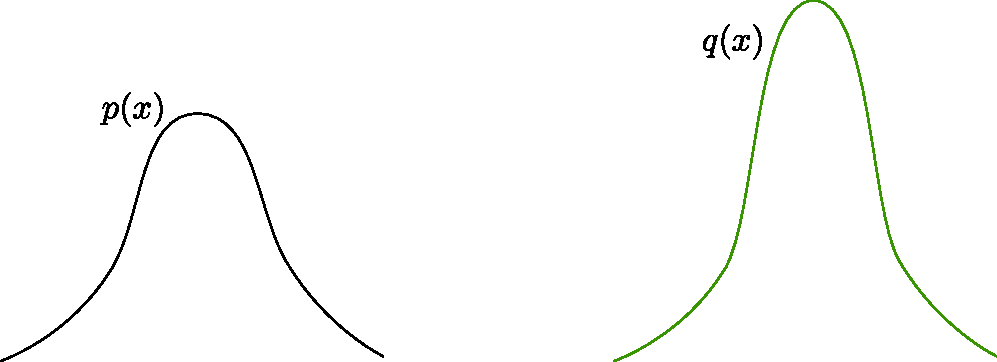
\includegraphics[scale=0.5]{./images/generative/gan/twodist.pdf}
	\end{center}
	\caption{Two distributions: $p(x)$ and $q(x)$}
	\label{fig:}
\end{figure}

Thus, both the forward KL and the reverse KL suffers an unstability issue. Specifically, in each case, if the denominator goes to zero, then the divergence goes to infinity. 

\subsection{Jensen-Shannon Divergence}

Definition:
$$D_{JS}(p_{data}||p_{G}) = \frac{1}{2}\Bigg[D_{KL}\Big(p_{data}\Big|\Big|\frac{p_{data}+p_{G}}{2}\Big)+D_{KL}\Big(p_{G}\Big|\Big|\frac{p_{data}+p_{G}}{2}\Big)\Bigg]$$

The KL divergence's issue can be alleviated by JS-divergence. Consider a simple example in Fig. \ref{fig:wassersteinexample}6
\begin{align*}
	\forall (x, y) \in P, x = 0 \text{ and } y \sim U(0, 1)\\
	\forall (x, y) \in Q, x = \theta, 0 \leq \theta \leq 1 \text{ and } y \sim U(0, 1)
\end{align*}

\begin{figure}[h]
	\begin{center}
		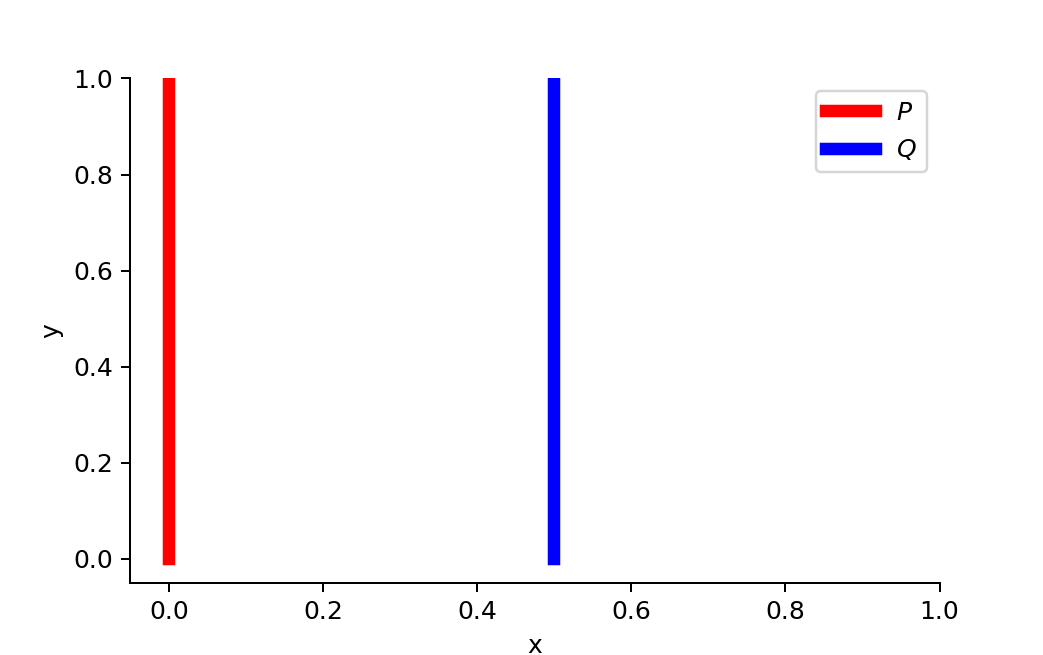
\includegraphics[scale=0.25]{./images/generative/gan/wassersteinexample.png}
	\end{center}
	\caption{Two distributions: $p(x)$ and $q(x)$}
	\label{fig:wassersteinexample}
\end{figure}

\begin{align*}
	D_\textrm{KL}(q(x)||p(x)) &= \infty\\
	D_\textrm{KL}(p(x)||q(x)) &= \infty\\
	D_{JS}(p_{data}||p_{G}) &= \frac{1}{2}\Bigg[D_{KL}\Big(p_{data}\Big|\Big|\frac{p_{data}+p_{G}}{2}\Big)+D_{KL}\Big(p_{G}\Big|\Big|\frac{p_{data}+p_{G}}{2}\Big)\Bigg]\\
	& = \frac{1}{2}\Bigg[D_{KL}\Big(p_{data}\Big|\Big|\frac{p_{data}}{2}\Big)++D_{KL}\Big(p_{G}\Big|\Big|\frac{p_{G}}{2}\Big)\Bigg]\\
	& = \frac{1}{2}[\log 2 + \log 2] = \log 2\\
	W(p,q) & = |\theta|
\end{align*}
Therefore, Jensen-Shannon divergence is more stabler than KL divergece. This is one of the reasons why GAN, which uses JS divergence works better than VAE, which uses KL divergence. 

However, JS divergence also has some problem. If the value is close to $\frac{1}{2}\log 2$, then the gradient will be very small or close to zero, because the divergence is close to constant. It means that a training speed is very slow. Thus, we need a better metric. 

\subsection{Wasserstein Distance}
Wasserstein Distance is a measure of the distance between two probability distributions. It is also called Earth Mover’s distance, short for EM distance, because informally it can be interpreted as the minimum energy cost of moving and transforming a pile of dirt in the shape of one probability distribution to the shape of the other distribution.
\begin{equation*}
	W(p_r, p_g) = \inf_{\gamma \sim \Pi(p_r, p_g)} \mathbbm{E}_{(x, y) \sim \gamma}[\| x-y \|]
\end{equation*}

\begin{itemize}
	\item $\Pi$: is the transportation plan and the set of all possible joint probability distributions between $p_r$ and $p_g$. One joint distribution $\gamma \sim \Pi(p_r, p_g)$ describes one transport plan.\
	\item $\mathbbm{E}_{x, y \sim \gamma} \| x-y \| = \sum_{x, y} \gamma(x, y) \| x-y \|$
	\item Finally, we take the minimum one among the costs of all dirt moving solutions as the EM distance (by infimum). 
\end{itemize}

\section{WGAN}
However, consider all possible joint distribution is intractable, so dual solution can be used. 

$$W(p_r, p_g) = \frac{1}{K} \sup_{\| f \|_L \leq K} \mathbbm{E}_{x \sim p_r}[f(x)] - \mathbbm{E}_{x \sim p_g}[f(x)]$$

So to calculate the Wasserstein distance, we just need to find a 1-Lipschitz function. To enforce the constraint, WGAN applies a very simple clipping to restrict the maximum weight value in $f$, i.e. the weights of the discriminator

Suppose this function $f$ comes from a family of $K$-Lipschitz continuous functions, $\{f_w\}_{w\in W}$, parameterized by $w$. In the modified Wasserstein-GAN, the ``discriminator'' model is used to learn $w$ to find a good $f_w$ and the loss function is configured as measuring the Wasserstein distance between $p_r$ and $p_g$.

$$L(p_r, p_g) = W(p_r, p_g) = \max_{w \in W} \mathbbm{E}_{x \sim p_r}[f_w(x)] - \mathbbm{E}_{z \sim p_r(z)}[f_w(g_\theta(z))]$$

There are two ways to satisfy the Lipschitz continuity:
\begin{itemize}
	\item Weight clipping
	\item Gradient Penalty
\end{itemize}

\subsection{Lipschitz continuity}
The function $f$ in the new form of Wasserstein metric is demanded to satisfy $\| f \|_L \leq K$, meaning it should be $K$-Lipschitz continuous. \citep{Lil2017}

A real-valued function $f: \mathbbm{R} \rightarrow \mathbbm{R}$ is called $K$-Lipschitz continuous if there exists a real constant $K\geq 0$ such that, for all $x_1, x_2 \in \mathbbm{R}$
$$\lvert f(x_1) - f(x_2) \rvert \leq K \lvert x_1 - x_2 \rvert$$
Here $K$ is known as a Lipschitz constant for function $f(\cdot)$. Functions that are everywhere continuously differentiable is Lipschitz continuous, because the derivative, estimated as $\frac{\lvert f(x_1) - f(x_2) \rvert}{\lvert x_1 - x_2 \rvert}$, has bounds. However, a Lipschitz continuous function may not be everywhere differentiable, such as $f(x) = \lvert x \rvert$

\begin{figure}[h]
	\begin{center}
		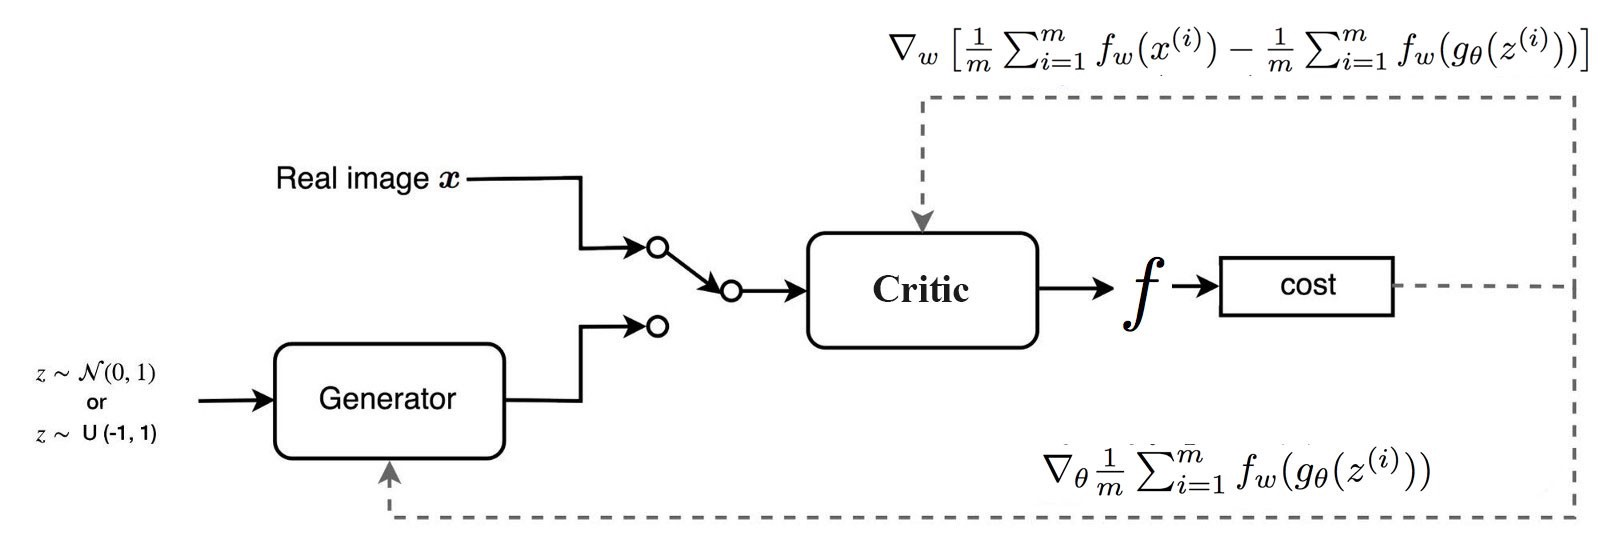
\includegraphics[scale=0.25]{./images/generative/gan/wgan.jpeg}
	\end{center}
	\caption{WGAN}
	\label{fig:wgan}
\end{figure}

\begin{figure}[h]
	\begin{center}
		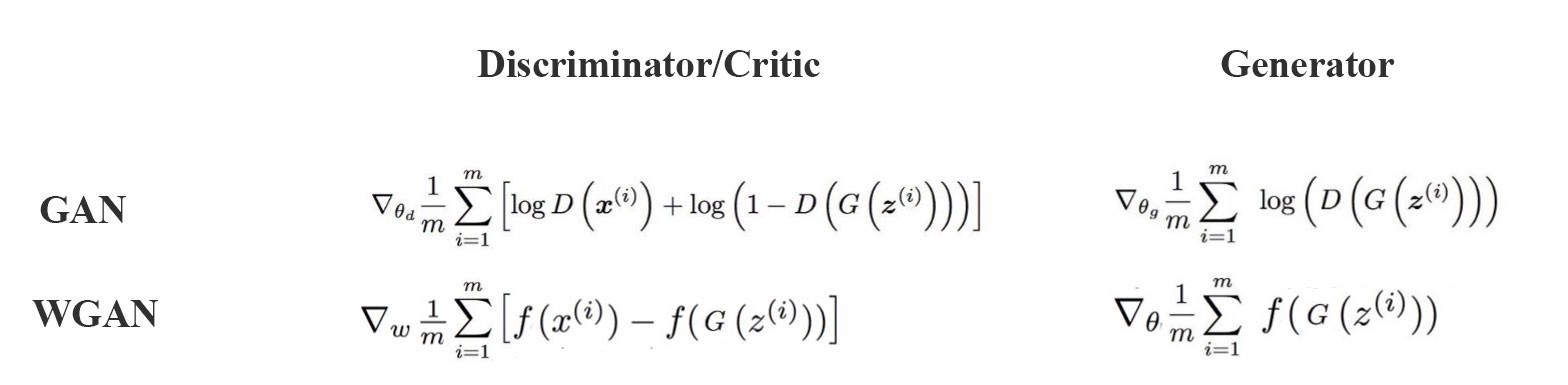
\includegraphics[scale=0.2]{./images/generative/gan/wgan_2.jpeg}
	\end{center}
	\caption{WGAN}
\end{figure}
